\subsection{Verifica}
\subsubsection{Obiettivi}
La verifica del prodotto garantisce che tutte le attività di processo compiute in un periodo di tempo del progetto, non abbiano introdotto errori nel prodotto. Per ogni prodotto intermedio che causa variazioni significative rispetto al precedente, è necessario compiere un processo di verifica. Avvenendo in passi intermedi, la verifica supporta la validazione finale del prodotto. Gli obiettivi di questo processo sono dunque:
\begin{itemize}
	\item rilevare la presenza di difetti nel prodotto per provi rimedio;
	\item assicurare che vengano rispettate i requisiti stabiliti per il sistema;
	\item aumentare la qualità del prodotto fornito.
\end{itemize}

\subsubsection{Attività}
\paragraph{Analisi statica}
\noindent L'analisi statica è un tipo di verifica effettuata senza la necessità di esecuzione del software. Esistono due metodi per attuare questo tipo di attività:
\begin{itemize}
	\item \textbf{Walkthrough:} verifica a "largo spettro" che analizza il prodotto in tutti i suoi aspetti. Non si basa su una conoscenza pregressa riguardo errori comuni, bensì sulla analisi totalitaria del prodotto, alla ricerca delle difformità e delle criticità. Proprio a causa di queste caratteristiche, è una metodologia di verifica che dispendiosa in termini di tempo;
	\item \textbf{Inspection:} differentemente dalla metodologia Walkthrough, l'Inspection si basa sull'esperienza. Conoscendo gli errori tipici durante i diversi periodi del ciclo di vita di un prodotto, è possibile stilare una lista di controllo e procedere ad analizzare i soli punti critici della struttura. Ogni qualvolta venga eseguita una verifica e vengano trovati nuovi punti critici per il controllo, si procede con l'aggiornamento della lista messa a disposizione di tutti i verificatori.
\end{itemize}
All'interno del \textit{Piano di Qualifica 2.0.0\doc} viene riportata la lista di controllo relativa al processo di documentazione.


\paragraph{Analisi dinamica}
L'analisi dinamica viene effettuata tramite l'ausilio di test. Ogni test per essere significativo, deve essere ripetibile. Per soddisfare tale richiesta, ogni test deve possedere le seguenti caratteristiche:
\begin{itemize}
	\item considera \textbf{l'ambiente} hardware e software di esecuzione;
	\item è caratterizzato da uno \textbf{stato iniziale};
	\item riceve in \textbf{input} dei valori;
	\item restituisce un \textbf{output} corrispondente con quello atteso;
	\item può contenere delle \textbf{istruzioni aggiuntive} sulle modalità di esecuzione del test e sulla loro interpretazione.
\end{itemize}

\subparagraph*{Modello a "V"}
\begin{figure}[h!]
	\caption{Schema del Modello a "V"}
	\centering
	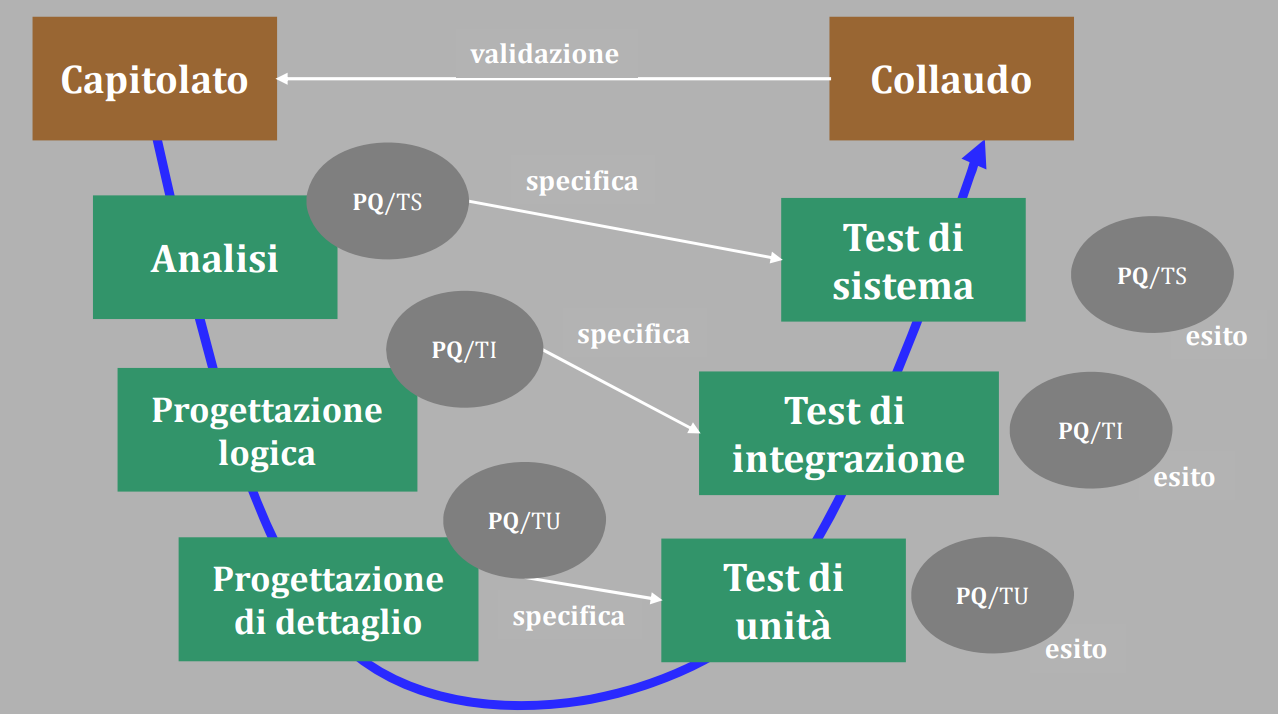
\includegraphics[width=\textwidth]{res/img/modelloV.png}
\end{figure}
Lo stato di integrazione di un prodotto software è rappresentabile in livelli, ognuno dei quali corrisponde ad una specifica revisione tecnica. Il modello a "V" rappresenta in maniera schematica la corrispondenza tra la tipologia di test e il livello del ciclo di vita software in cui essi vengono eseguiti. A ognuno di questi livelli, corrisponde una tipologia di test specifica. A partire dall'implementazione con i test di unità, si effettuano verifiche del prodotto sempre più complete sino ad arrivare al collaudo finale.

\subparagraph*{Test di unità}
Vengono effettuate delle prove sulle unità che compongono il prodotto software. Le unità rappresentano la più piccola parte del prodotto che è possibile eseguire e verificare autonomamente. Questa tipologia di test è effettuata con l'ausilio degli \textit{stub\glo} e dei \textit{driver\glos}.

\subparagraph*{Test di integrazione}
Test che agiscono a livello di componente. Possono essere eseguiti solo su un insieme di unità precedentemente testate. Il compito dei test di integrazione è di verificare se le unità presentano il comportamento atteso quando operano insieme a livello di componente.

\subparagraph*{Test di sistema} 
Si basano sull'intero sistema e hanno lo scopo di verificare del funzionamento del prodotto dopo l'assemblamento delle varie componenti che lo costituiscono. Essi dovranno verificare i requisiti definiti nell'\textit{Analisi dei requisiti 1.0.0\docs}.

\subparagraph*{Test di accettazione}
Verificano il prodotto nella sua completezza e si basano sull'esperienza del cliente rispetto ai bisogni espressi nel \textit{capitolato\glos}.

\subparagraph*{Test di regressione}
Vengono effettuati a seguito di una modifica apportata al sistema. Ogni modifica deve essere necessariamente seguita dall'esecuzione di tutti i test esistenti. Ciò servirà per accertare che la correttezza della modifica effettuata. 


\subsubsection{Procedure}
\paragraph{Verifica della documentazione mediante inspection}
\begin{enumerate}
	\item ispezionare il documento o parte di esso seguendo i punti critici rilevati dalla tabella;
	\item notificare al responsabile della stesura del documento gli errori commessi;
	\item aggiornare la tabella degli errori comuni: se durante la verifica sono state rilevate delle ricorrenze per delle tipologie di errori non presenti all'interno della lista, dovranno essere riportate.
\end{enumerate}
\paragraph{Ottenimento e gestione esiti misurazioni}
\begin{enumerate}
	\item scegliere la metrica coinvolta per la misurazione della qualità di processo e di prodotto;
	\item calcolare il valore corrispondente all'avvenuta misurazione;
	\item verificare l'esito in base al risultato ottenuto;
	\item inserire i risultati ottenuti all'interno di un grafico che metta lo metta a paragone con quelli rilevati negli incrementi precedenti;
	\item inserire il grafico in appendice del PdQ. 
\end{enumerate}

\subsubsection{Strumenti}
\paragraph{ESLint}
Strumento di analisi del codice utilizzato per lo sviluppo in JavaScript. Consente la creazione di codice leggibile e coerente con regole condivise dalla comunità degli sviluppatori. Esso è semplicemente installabile come \textit{plug-in\glo} di Visual Studio Code oppure mediante npm. 

\paragraph{Mocha}
Framework per eseguire unit testing in linguaggio Typescript e per gli \textit{smart contract\glo} scritti in Solidity. Il framework è supportato da Visual Studio Code.
